%%%%%%%%%%%%%%%%%%%%%%%%%%%%%%%%%%%%%%%%%%%
% Masters/Doctoral Thesis 
% LaTeX Template
% Version 1.42 (19/1/14)
%v 
% This template has been downloaded from:
% http://www.latextemplates.com
% Original authors:
% Steven Gunn 
% http://users.ecs.soton.ac.uk/srg/softwaretools/document/templates/
% and
% Sunil Patel
% http://www.sunilpatel.co.uk/thesis-template/
%
% License:
% CC BY-NC-SA 3.0 (http://creativecommons.org/licenses/by-nc-sa/3.0/)
%
% Note:
% Make sure to edit document variables in the Thesis.cls file
%
%%%%%%%%%%%%%%%%%%%%%%%%%%%%%%%%%%%%%%%%%

%----------------------------------------------------------------------------------------
%	PACKAGES AND OTHER DOCUMENT CONFIGURATIONS
%----------------------------------------------------------------------------------------

\documentclass[12pt, letterpaper, twoside, openright]{Thesis} % Paper size, default font size and one-sided paper
\usepackage{pdfpages}
\usepackage{subcaption}
\graphicspath{{Pictures/}} % Specifies the directory where pictures are stored
\usepackage[square, numbers, comma, sort&compress]{natbib} % Use the natbib reference package - read up on this to edit the reference style; if you want text (e.g. Smith et al., 2012) for the in-text references (instead of numbers), remove 'numbers' 
\usepackage[spanish,english]{babel}
\hypersetup{urlcolor=blue, colorlinks=true} % Colors hyperlinks in blue - change to black if annoying
\title{\ttitle} % Defines the thesis title - don't touch this
\appendix % Cue to tell LaTeX that the following 'chapters' are Appendices

% Include the appendices of the thesis as separate files from the Appendices folder
% Uncomment the lines as you write the Appendices

%% Appendix A

\chapter{Codes} % Main appendix title

\label{codes} % For referencing this appendix elsewhere, use \ref{AppendixA}

\lhead{Appendix A. \emph{Codes}} % This is for the header on each page - perhaps a shortened title

\section{Run Synrad3d}
\begin{verbatim}
k=simulation_1
./sendbatchs verylong $k /afs/cern.ch/work/g/gerardo/bmad_dist/bsim/synrad3d ./synrad3d synrad.init
\end{verbatim}

\section{Batch}
\begin{verbatim}
jobpath=/afs/cern.ch/user/g/gerardo/scratch1/
sourcepath=/afs/cern.ch/user/g/gerardo/synrad3d
current=`pwd`

  if [ $# -ne '0' ]
  then

count=$2
limit=$2

	jobname="/$3 > $jobpath$count/output.data"
	echo $jobpath$count
	mkdir $jobpath$count
	cp $sourcepath/job$1.nqb $jobpath$count/jobscript.nqb
	cp $current/$4 $jobpath$count/ecloud.input
    cd $jobpath$count
	echo "#BSUB -J inel3 " >> jobscript.nqb
	echo "#BSUB -o $jobpath$count/job.output" >> jobscript.nqb
	echo "#BSUB -e $jobpath$count/err.output" >> jobscript.nqb
	echo "cd $jobpath$count" >> jobscript.nqb

    echo $sourcepath$jobname >> jobscript.nqb
	echo "cp eloss.data $jobpath$count" >> jobscript.nqb
	echo "cp main.data $jobpath$count" >> jobscript.nqb
	echo "cp *.output $jobpath$count" >> jobscript.nqb
	echo "cp err*.* $jobpath$count" >> jobscript.nqb

    bsub < $jobpath$count/jobscript.nqb


  else
   echo "Please specify a job class (short, medium or long)"
   echo "a run number, an executable and an include file!"
   echo "Usage: sendbatch 'class' 'runnumber' 'exec' 'include file'"
  fi
\end{verbatim}

%\input{Appendices/AppendixB}
%\input{Appendices/AppendixC}


\addtocontents{toc}{\vspace{2em}} % Add a gap in the Contents, for aesthetics

\backmatter

%----------------------------------------------------------------------------------------
%	BIBLIOGRAPHY
%----------------------------------------------------------------------------------------

\label{Bibliography}
%\renewcommand{\refname}{References}  % for the article class
\renewcommand{\bibname}{References}  % for the report or book class

\lhead{\emph{References}} % Change the page header to say "Bibliography"

\bibliographystyle{unsrtnat} % Use the "unsrtnat" BibTeX style for formatting the Bibliography

\bibliography{Bib} % The references (bibliography) information are stored in the file named "Bibliography.bib"





\begin{document}

\frontmatter % Use roman page numbering style (i, ii, iii, iv...) for the pre-content pages

\setstretch{1.3} % Line spacing of 1.3
	
% Define the page headers using the FancyHdr package and set up for one-sided printing
\fancyhead{} % Clears all page headers and footers
\rhead{\thepage} % Sets the right side header to show the page number
\lhead{} % Clears the left side page header

\pagestyle{fancy} % Finally, use the "fancy" page style to implement the FancyHdr headers
\newcommand{\srthree}{\texttt{Synrad3D}\xspace}
\newcommand{\HRule}{\rule{\linewidth}{0.5mm}} % New command to make the lines in the title page

% PDF meta-data
\hypersetup{pdftitle={\ttitle}}
\hypersetup{pdfsubject=\subjectname}
\hypersetup{pdfauthor=\authornames}
\hypersetup{pdfkeywords=\keywordnames}

%----------------------------------------------------------------------------------------
%	TITLE PAGE
%----------------------------------------------------------------------------------------
%\begin{titlepage}


%\end{titlepage}
%----------------------------------------------------------------------------------------
%	DECLARATION PAGE
%	Your institution may give you a different text to place here
%----------------------------------------------------------------------------------------

\Declaration{

\addtocontents{toc}{\vspace{1em}} % Add a gap in the Contents, for aesthetics

I, \authornames, declare that this thesis titled, '\ttitle' and the work presented in it are my own. I confirm that:

\begin{itemize} 
\item[\tiny{$\blacksquare$}] This work was done wholly or mainly while in candidature for a research degree at CINVESTAV.
\item[\tiny{$\blacksquare$}] Where any part of this thesis has previously been submitted for a degree or any other qualification at CINVESTAV or any other institution, this has been clearly stated.
\item[\tiny{$\blacksquare$}] Where I have consulted the published work of others, this is always clearly attributed.
\item[\tiny{$\blacksquare$}] Where I have quoted from the work of others, the source is always given. With the exception of such quotations, this thesis is entirely my own work.
\item[\tiny{$\blacksquare$}] I have acknowledged all main sources of help.
\item[\tiny{$\blacksquare$}] Where the thesis is based on work done by myself jointly with others, I have made clear exactly what was done by others and what I have contributed myself.\\
\end{itemize}
 
Signed:\\
\\
\rule[1em]{25em}{0.5pt} % This prints a line for the signature
\\
Gerardo Guillermo
 
Date: \today \\
\rule[1em]{25em}{0.5pt} % This prints a line to write the date
}

\clearpage % Start a new page

%----------------------------------------------------------------------------------------
%	QUOTATION PAGE
%----------------------------------------------------------------------------------------

\pagestyle{empty} % No headers or footers for the following pages

\null\vfill % Add some space to move the quote down the page a bit

\textit{``God used beautiful mathematics in creating the world."}

\begin{flushright}
Paul Dirac
\end{flushright}

\vfill\vfill\vfill\vfill\vfill\vfill\null % Add some space at the bottom to position the quote just right

\clearpage % Start a new page

%----------------------------------------------------------------------------------------
%	ABSTRACT PAGE
%----------------------------------------------------------------------------------------

\addtotoc{Abstract} % Add the "Abstract" page entry to the Contents

\abstract{\addtocontents{toc}{\vspace{1em}} % Add a gap in the Contents, for aesthetics

At energies in the order of TeV, synchrotron radiation (SR) is very high, even in a hadron beam. SR could be regarded as an important heat load to the cryogenic system cooling the superconducting electromagnets. In this work SR is simulated using \srthree to analize which lattice elements of a section of the LHC absorb the most photon and analize how does it affect to have a sawtooth pattern in the beam screen.
}

\addtotoc{Resumen} % Add the "Abstract" page entry to the Contents
\selectlanguage{spanish}
\abstract{\addtocontents{toc}{\vspace{1em}} % Add a gap in the Contents, for aesthetics
A energías en el orden de TeV la radición de sincrotrón es muy alta, incluso usando rayos de hadrones, esta radiación puede representar una carga calórica demasiado grande para electroimanes trabajando en estado criogénico. En este trabajo se simula la radiación de sincrotrón generada por un haz de protones en el LHC, utilizando \srthree, para analizar qué sección en un arco absorben la mayor cantidad de fotones y analizar como nos afecta tener en la pantalla ('beam screen') un patrón de diente de sierra.
}
\selectlanguage{english}
\clearpage % Start a new page

%----------------------------------------------------------------------------------------
%	ACKNOWLEDGEMENTS
%----------------------------------------------------------------------------------------

\setstretch{1.3} % Reset the line-spacing to 1.3 for body text (if it has changed)

\acknowledgements{\addtocontents{toc}{\vspace{1em}} % Add a gap in the Contents, for aesthetics

I cannot express enough thanks to the members of this thesis committee: Dr. Rodrigo Huerta Quintanilla and Dr. Román Castro Rodriguez.

The completion of this project could not have been accomplished without the support of my supervisor, Jesus Guillermo Contreras Nuño; and so many people at CERN specially Frank Zimmermann.

I thank Consejo de Ciencia y Tecnología (CONACYT) and CINVESTAV for the financial support during my masters studies. I also thank CERN for all the information they make available to students such as myself.

I also want to thank the administrative personnel from CINVESTAV Mérida which has been helpful and efficient, specially Dr. Gerko Oskam and Zhirnay Rodriguez Pinelo.
}
\clearpage % Start a new page


%----------------------------------------------------------------------------------------
%	LIST OF CONTENTS/FIGURES/TABLES PAGES
%----------------------------------------------------------------------------------------

\pagestyle{fancy} % The page style headers have been "empty" all this time, now use the "fancy" headers as defined before to bring them back

\lhead{\emph{Contents}} % Set the left side page header to "Contents"
\tableofcontents % Write out the Table of Contents

\lhead{\emph{List of Figures}} % Set the left side page header to "List of Figures"
\listoffigures % Write out the List of Figures

\lhead{\emph{List of Tables}} % Set the left side page header to "List of Tables"
\listoftables % Write out the List of Tables

%----------------------------------------------------------------------------------------
%	ABBREVIATIONS
%----------------------------------------------------------------------------------------

\clearpage % Start a new page

\setstretch{1.5} % Set the line spacing to 1.5, this makes the following tables easier to read

\lhead{\emph{Abbreviations}} % Set the left side page header to "Abbreviations"
\listofsymbols{ll} % Include a list of Abbreviations (a table of two columns)
{
\textbf{AFS} & \textbf{A}ndrew \textbf{F}ile \textbf{S}ystem \\
\textbf{ALICE} & \textbf{A} \textbf{L}arge \textbf{I}on \textbf{C}ollider \textbf{E}xperiment\\
\textbf{ATLAS} & \textbf{A} \textbf{T}oroidal \textbf{L}HC \textbf{A}pparatu\textbf{S}\\
\textbf{CERN} & \textbf{C}onseil \textbf{E}uropéen pour la \textbf{R}echerche \textbf{N}ucléaire\\
 & European Organization for Nuclear Research  \\ 
\textbf{CFH} & \textbf{C}onfoederatio \textbf{H}elvetica \textbf{F}ranc\\
\textbf{CMS} & \textbf{C}ompact \textbf{M}uon \textbf{S}olenoid\\
\textbf{FODO} & \textbf{Fo}ocus$/$\textbf{D}ef\textbf{O}cus\\
\textbf{LHC} & \textbf{L}arge \textbf{H}adron \textbf{C}ollider \\
\textbf{LHCb} & \textbf{LHC} \textbf{b}eauty		 \\
\textbf{LEP} & \textbf{L}arge \textbf{E}lectron - \textbf{P}ositron Collider \\
\textbf{LxPLUS} & \textbf{L}x \textbf{P}ublic \textbf{L}ogin \textbf{S}ervice\\
\textbf{SLC5} & \textbf{S}cientific \textbf{L}inux \textbf{C}ERN \textbf{5}\\
\textbf{SMIF} & \textbf{S}ynrad3D \textbf{M}ain \textbf{I}nput \textbf{F}ile\\
\textbf{SMOF} & \textbf{S}ynrad3D \textbf{M}ain \textbf{O}utput \textbf{F}ile\\
\textbf{SR} & \textbf{S}ynchrotron \textbf{R}adiation \\
\textbf{SSS} & \textbf{S}hort \textbf{S}traight - \textbf{S}ection \\
%\textbf{LHC} & \textbf{L}arge \textbf{H}adron \textbf{C}ollider \\
%\textbf{Acronym} & \textbf{W}hat (it) \textbf{S}tands \textbf{F}or \\
}

%----------------------------------------------------------------------------------------
%	PHYSICAL CONSTANTS/OTHER DEFINITIONS
%----------------------------------------------------------------------------------------

%\clearpage % Start a new page
%
%\lhead{\emph{Physical Constants}} % Set the left side page header to "Physical Constants"

%\listofconstants{lrcl} % Include a list of Physical Constants (a four column table)
%{
%Speed of Light & $c$ & $=$ & $2.997\ 924\ 58\times10^{8}\ \mbox{ms}^{-\mbox{1}}$ (exact)\\
%Electron Volt & $c$ & $=$ & $1.602\ 176\ 57\times10^{-19}\ \mbox{J}$ (exact)\\
% Constant Name & Symbol & = & Constant Value (with units) \\
%}

%----------------------------------------------------------------------------------------
%	SYMBOLS
%----------------------------------------------------------------------------------------

\clearpage % Start a new page

\lhead{\emph{Symbols}} % Set the left side page header to "Symbols"

\listofnomenclature{lll} % Include a list of Symbols (a three column table)
{
$d$ & Distance & m \\
$E$ & Energy & eV \\
$P$ & Power & W (Js$^{-1}$) \\
$s$ & Transversal Direction & m \\
$T$ & Temperature & K \\
% Symbol & Name & Unit \\

& & \\ % Gap to separate the Roman symbols from the Greek
$\gamma_r$ &  Relativistic gamma factor & \\
$\varepsilon_{c}$ & Critical photon energy & eV \\
$\rho$ & Radius & m \\
$\sigma$ & Surface roughness & nm \\
$\omega_{c}$ & Critical photon frequency & rads$^{-1}$ \\

% Symbol & Name & Unit \\
}

%----------------------------------------------------------------------------------------
%	DEDICATION
%----------------------------------------------------------------------------------------

%\setstretch{1.3} % Return the line spacing back to 1.3

%\pagestyle{empty} % Page style needs to be empty for this page

%\dedicatory{Dedicated to my imaginary girlfriend, who has always been my motivator} % Dedication text

%\addtocontents{toc}{\vspace{2em}} % Add a gap in the Contents, for aesthetics

%----------------------------------------------------------------------------------------
%	THESIS CONTENT - CHAPTERS
%----------------------------------------------------------------------------------------

\mainmatter % Begin numeric (1,2,3...) page numbering

\pagestyle{fancy} % Return the page headers back to the "fancy" style

% Include the chapters of the thesis as separate files from the Chapters folder
% Uncomment the lines as you write the chapters

% Chapter 1

\chapter{Introduction} % Main chapter title

\label{intro} % For referencing the chapter elsewhere, use \ref{Chapter1} 

\lhead{Chapter 1. \emph{Introduction}} % This is for the header on each page - perhaps a shortened title

In every circular particle accelerator, such as the LHC, energy is emitted in the form of synchrotron radiation (SR). This energy is then absorbed by the machine protection system. A circular accelerator consists mostly of 'superbends', electromagnets built with superconductor materials, which need to be very cold (around 4 K). If the LHC superbends heat up from 1.9 K to 4.5 K, the magnetic field strength decreases from 8.33 T to 6.8 T\citep{faq}. SR from bunches in the LHC creates electrons by photoelectric effect at the vacuum chamber wall. These electrons are accelerated by the positively charged particle bunch; when they impact the opposite wall, they can generate secondary electrons which can in turn be accelerated by the next bunch. Therefore, and avalanche production of secondary electrons gives rise to an electron cloud and its undesirable effects\citep{miguel}. This is the reason why it is so important to know where and how SR is absorbed by each element of the lattice that conforms the accelerator.

At the LHC the maximum $\gamma_r = [1 - (\frac{v_r}{c})^{2}]^{-1/2}$ that can be reached depends on the maximum magnetic dipole field, which nominally is 8.33 T at 7 TeV beam energy, but the actual field limit depends on the heat load and temperature of the magnets and therefore on the amount of the radiation of the machine during operation\citep{DR}. So to achieve higher dipole fields we need to minimize the effects of SR.

It is not common that SR is considered as a problem in hadron storage rings, because it is very small compared to electron storage rings, but at very high energies such as the ones reached at the LHC it becomes a problem specially when it is then absorbed by the cryogenic system\citep{DR}.

Work on this matter has been done by D. Sagan, G. Duncan, F. Zimmermann and G.H.I Maury\citep{TUP}. In this thesis, we continue and extend the studies of \citep{TUP}. These studies consist on the use of  \srthree code, described in \ref{Synrad3d}, to track SR photons at the LHC ring. Their simulations were performed for a 7 TeV proton beam energy and assumed a C layer of 10 nm on a Cu substrate. We study this problem in very particular conditions: at the LHC at CERN we focus on the main bending elements elements and we are adding the sawtooth pattern, a series of 30 $\mu$m high steps spaced at a distance of 500 $\mu$m in the longitudinal direction which is impressed on the horizontal outer side of the beam screen. Through simulation using the simulation software \srthree , we are able to tell which element absorb the largest number of photons and  how many times did the photons bounce before being absorbed.

The main objective of this work is to analyze the difference in the simulation between using the sawtooth pattern or not in a small section of the main bending magnets with a 7 TeV proton energy beam. 

%----------------------------------------------------------------------------------------

%\section{sexion}

% Chapter Template

\chapter{Fundamentals on Synchrotron Radiation} % Main chapter title

\label{sr} % Change X to a consecutive number; for referencing this chapter elsewhere, use \ref{ChapterX}

\lhead{Chapter 2. \emph{Fundamentals on Synchotron Radiation}} % Change X to a consecutive number; this is for the header on each page - perhaps a shortened title

We call synchrotron radiation to the energy emitted by a charge which has a radial acceleration. It is produced in circular accelerators such as the LHC.
%----------------------------------------------------------------------------------------
%	SECTION 1
%----------------------------------------------------------------------------------------

\section{Radiation}
\begin{figure}
	\centering
  \begin{minipage}{\textwidth}
  	\centering
   	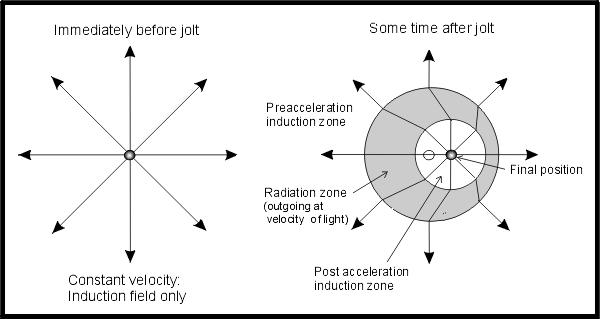
\includegraphics[width=3.5in]{Pictures/efields.jpg}
  		\caption{\label{fig:campos}
   			Electromagnetic field of a charge a) static b)after a short jolt }
   			\footnotesize{Picture taken from on \citep{img1}}
   \end{minipage}
\end{figure}
The idea of electromagnetic waves has always fascinated the mind of physicists around the world. In 1887 G. Hertz generated, emitted and received electromagnetic waves. This was an experimental proof of Maxwell's equations. The source of that radiation were oscillating charges.

First of all we should know that electromagnetic radiation is a consecuence of the finite velocity of light\citep{libro}. While a particle is at rest, or in a constant motion, it emits electric field lines radially out to infinity. If we suddenly accelerate this charge, the information of that acceleration travels with the speed of light, so that information is only known to the vicinity defined by: \begin{equation}
\Delta d \leq c* \Delta t  
\end{equation}
The distortion of these lines, which is traveling away from the charge is what we call electromagnetic radiation. This concept is shown in Figure \ref{fig:campos}.

\subsection{Conservation Laws}
The emission of electromagnetic radiation from free electrons is a classical phenomenon. We may therefore use a visual approach to gain some insight into conditions and mechanisms of radiation emission.
The emission of electromagnetic radiation involves two components, the electron and the radiation field. For the combined system energy–momentum conservation must be fulfilled. These conservation laws impose very specific selection rules on the kind of emission processes possible.
%-----------------------------------
%	SUBSECTION 2
%-----------------------------------
\section{Synchrotron Radiation}
The interest in electromagnetic theory grew in the mid 1940s with the development of the free electron radiation theories, mainly  because of the development of circular high energy electron accelerators. In 1944 Pomeranchouk showed that there was a limit to the betatron principle, and that there was also an energy limit due to the losses from electromagnetic radiation. The energy that charged particles lose to SR posed technological and economic problems to increase circular accelerators maximum energy. To surpass this limitation, circular accelerators started growing diametrically\citep{libro}.

When a relativistic beam of charged particles changes direction, it emits electromagnetic radiation, that can be seen as a search light, because it is highly collimated in the forward direction although it is broadband radiation, this is shown in Figure \ref{fig:synsim}. The shortness of this pulse is what indicates the observer it has detected synchrotron radiation with a broadband spectrum which is characterized by the critical photon energy. This energy depends solely on the paticle's energy and its bending radius as shown in equation \ref{eq:critical energy}, where $\varepsilon_{c}$ is the critical photon energy, $\omega_{c}$ is the critical photon frequency, $E$ is the particle's energy, and $\rho$ is the bending radius\citep{libro}. 
\begin{equation}
\label{eq:critical energy}
\varepsilon_{c} = \hbar\omega_{c} = \dfrac{3\hbar c}{2(mc^{2})^{3}}\dfrac{E^{3}}{\rho}
\end{equation}

There are particular characteristics of synchrotron radiation that depend on the magnetic devices used to generate that radiation, such as wigglers, undulators, wavelength shifters, etc. Nevertheless in this work we are only interested in bending magnets, furthermore superbends.

\begin{figure}
	\centering
  \begin{minipage}{\textwidth}
  	\centering
   	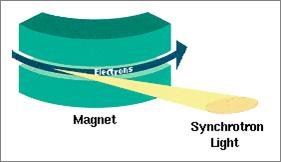
\includegraphics[width=3.5in]{Pictures/Syncrotron.jpg}
  		\caption{\label{fig:synsim}
   			Synchrotron radiation produced by a bending magnet.}
   			\footnotesize{Picture taken from \citep{fig:wiki1}}
   \end{minipage}
\end{figure}

\subsection{Superbends}
When a charged particle enters a magnetic field region, the particle is  deflected from its original trajectory perpendicularly to the magnetic field. The radius of this deflection depens only on the energy of the particle, its charge and the strength of the field. So we can express the critical photon energy as a function of the particle energy and the magnetic field. The numerical expression for an electron is shown in equation \ref{eq:51}\citep{libro}. 

\begin{equation}
\label{eq:51}
\varepsilon_{c}(keV) = 2.2183\dfrac{E^{3}(GeV^{3})}{\rho(m)}=0.66503E^{2}(GeV)B(T) 
\end{equation}

Where $B$ is the strength of the field. Sometimes the critical energy required for a given experiment is too high to be reached using regular magnets, or if we have a fixed $\rho$ and try to achieve maximum particle energy, as is the case of the LHC which had to fit in the LEP tunnel as mentioned in chapter \ref{ch:LHC}. In those cases regular magnets are replaced with much stronger and shorter superconducting electromagnets. Conventional bending magnet fields rarely exceed 1.5 T, but superconducting magnets can be operated at 5 to 6 T or higher\citep{libro}


%-----------------------------------
%	SUBSECTION 2
%-----------------------------------

\section{Radiation Power}
To know the total radiated power we integrate the Poynting vector $\vec{S}$ over a closed surface that keeps the charge inside. 
\begin{equation}
\label{eq:24}
P=\oint \vec{S}\cdot d\vec{A} 
\end{equation}
Doing this we find that the power radiating from a charged particle moving perpendicularly to a magnetic field is proportional to the fourth power of the particle's momentum and inversely proportional to the square of the bending radius\citep{libro}. For that reason, a slight increase in energy for a high energy particle leads to a huge increase of power loss due to synchrotron radiation. This is the reason why highest energy particle accelerators require a very large diameter.


%----------------------------------------------------------------------------------------
%	SECTION 2
%----------------------------------------------------------------------------------------


 
% Chapter 3

\chapter{LHC} % Main chapter title

\label{ch:LHC} % For referencing the chapter elsewhere, use \ref{Chapter1} 

\lhead{Chapter 3. \emph{LHC}} % This is for the header on each page - perhaps a shortened title

%----------------------------------------------------------------------------------------
The Large Hadron Collider (LHC) at CERN is a wonder of engineering and technology. It lies inside a 26.7 Km circular tunnel and 100 meters under the ground. Its construction took over 15 years, involved engineers from all over the world and costed over 6.5 billion CHF. Inside the tunnel there are two counter-rotating hadron beams accelerated to energies up to 7 TeV each. This beams are then forced to collide inside four huge detectors that measures the products of the collision\citep{LHCMT}.
\section{Characteristics}
The 26,659 m tunnel used by the LHC was inherited from the LEP, when it was shut down. The basic layout consists of eight long straight sections and eight bending arcs\citep{keil}. In order to keep the 7 TeV proton beams in such a small orbit it was necessary to use 1,232 magnets with a 8.3 T field that extend to a length of 14.3 m each\citep{DR}. To achieve this, powerful magnetic field superconducting magnets were to be used. Because of commercial availability NbTi superconductors were used, this material needs to be cooled down below 4.2 K to reach the superconducting state.
The solution was, and still is, to keep the magnets submerged in superfluid Helium below 2 K\citep{keil}.
The basic layout is shown in Figure \ref{Schem}, where Beam 1 is shown in blue and circulates clockwise; and in red Beam 2 which  rotates counterclockwise. There are four intersections, one in each major experiment: ATLAS, CMS, LHC-b, and ALICE. The first two, ATLAS and CMS, are high luminosity experiments and are located diametrically opposite to each other, while LHC-b is an devoted to quark b experiments, and ALICE stands for A Large Ion Collider Experiment, which is self-explanatory and work with full stripped Pb ions. The LHC consist of 8 arcs and 8 straight section and it is divided in octants, that start at the center of on arc and end at the center of the next one\citep{DR}. 
\begin{figure}
	\centering
  \begin{minipage}{\textwidth}
  	\centering
   	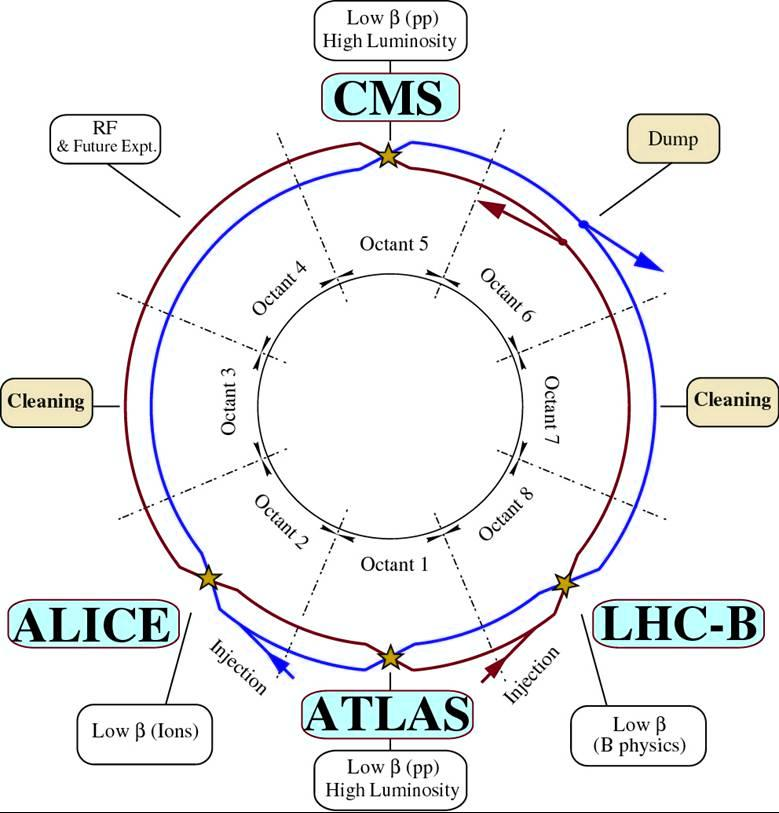
\includegraphics[width=3.5in]{Pictures/imagen.jpg}
  		\caption{\label{Schem}
   			General schematic for the LHC}
   			\footnotesize{Picture courtesy of CERN.}
   \end{minipage}
\end{figure}
The main parameters when working at its maximum energy are listed in Table \ref{table:LHCparam}. 
\begin{table}%[ht]
%\centering % used for centering table
\caption{Main parameters for proton-proton collisions} % title of Table
\begin{minipage}{\textwidth}
\renewcommand{\thefootnote}{\thempfootnote}

%\footnote{This table was taken from "the LHC vacuum system", p. 292 \citep{vacuum}. }
\begin{tabular}{l c}% centered columns (4 columns)
\hline
Energy \hspace{8.5cm} & 7 TeV \\ % inserting body of the table
Dipole Field & 8.33 T \\
coild aperture & 56 mm \\
Luminosity &10\textsuperscript{34} s\textsuperscript{$-$1} cm\textsuperscript{$-$2} \\
Injection energy & 450 GeV \\
Circulating current/beam & 0.56 A\\
Bunch spacing & 25 ns \\
Particles/bunch & 1.1$\times$10\textsuperscript{11} \\
Stored beam energy & 350 MJ \\
Normalised trasverse emittance & 3.75 $\mu$m \\
RMS bunch length & 0.075 m \\
Beam lifetime & 22 h \\
Luminosity lifetime & 10 h \\
Energy loss/turn & 6.7 keV \\
Critical photon energy & 45 eV \\
Linear photon flux & 1$\times$10\textsuperscript{17} m\textsuperscript{$-$1}s\textsuperscript{$-$1} \\
Total radiated power/beam & 3.8 kW \\ [1ex] % [1ex] adds vertical space
\hline
\end{tabular}
\end{minipage}
\begin{minipage}{\textwidth}
\begin{footnotesize}
* This table was taken from "the LHC vacuum system", p. 292 \citep{vacuum}.
\end{footnotesize}
\end{minipage}
\label{table:LHCparam} % is used to refer this table in the text
\end{table}

\subsection{Arc Cells}
The arcs consist of 23 regular arc cells. These are made out of two 53.45 m long half cells each of which consist of one cold mass with a length of 5.355m (6.63 mlong cryostat) short straight section (SSS) assembly and three 14.3 m long dipole magnets. The optics of Beam 1 and Beam 2 are coupled by electrical connections of the main magnets. There is also a dispersion suppressor at every transition between arcs and straight sections. The arc cells emulate a FODO lattice\citep{DR}.
\subsection{Optics}
The LHC optics design allows an optics matching with fixed and equal phase advances over the insertion regions for both beams that does not perturb the optics in the rest of the machine. The total number of particle trajectory oscillations during one revolution in the storage ring of the machine is adjusted by the optics of the arc cell. The flexibility of the phase advance over the insertions provides a measure for the flexibility of the total LHC optics and tell us how much liberty we have to change the phase advance between the main experimental insertions\cite{DR}.

\subsection{LHC Beam Pipe}
Because of the high beam intensities given by luminosities such as the one shown in Table \ref{table:LHCparam}, the LHC cannot work the same way as the Tevatron, which uses a single vacuum chamber and one set of magnets for both beams, the LHC requieres a vacuum chamber and set of magnets for each beam, and the beams only share the regions where the collisions take place and are around 130 m long\citep{DR}.
On one hand we have the price of the magnets and on the other hand we have the problem that there is not enough space in the LEP tunnel for two sets of magnets; as a result the LHC was built with twin bore magnets constructed of two sets of coils and beam channels within the same mechanical structure and cryostat\citep{DR}.

\textcolor{black}{90\% of the LHC surface should be maintained below 20 K and is made of copper cladded stainless steel in order to reduce ohmic resistence. The rest can stay at room temperature and is made of thick copper beam pipe \citep{DR}.}


\label{screen}
Another important feature of the beam pipe is the beam screen, this is a cooled screen intended to intercept SR at temperatures higher than 1.9 K and electrons due to electron clouds in order to prevent the magnets from heating. Figure \ref{fig:screen} shows the conceptual design of the LHC beam screen\citep{DR}\citep{vacuum}. 
\textcolor{black}{
The manufacturing process starts by co-laminating a specially developed low permeability 1mm thick
austenitic stainless steel strip with a 75 $\mu$m copper sheet and rolling a saw-tooth structure which  will intercept photons at normal incidence, thereby reducing the amount of reflected photons. The pumping slots are punched into this composite strip, which is then rolled into its final shape and closed by a longitudinal
weld\citep{vacuum}.
}
\begin{figure}
	\centering
  \begin{minipage}{\textwidth}
  	\centering
   	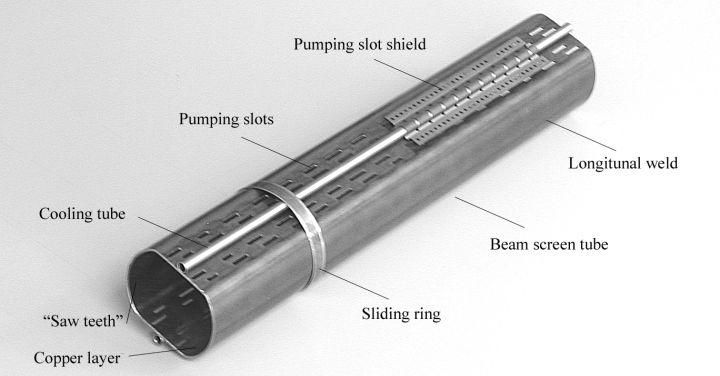
\includegraphics[width=3.5in]{Pictures/screen.png}
  		\caption{\label{fig:screen}
   			LHC Beam Screen}
   			\footnotesize{Picture courtesy of CERN.}
   \end{minipage}
\end{figure}

\subsection{Cryogenics}
\label{cryo}
The LHC uses cryomodules that consume liquid helium and expel evaporated helium. Each module looses 150 W statically in addition to the dynamic losses, that span from 100 W to 800 W.
For operation at nominal field the pressure inside the helium tank has to be carefully controlled to avoid frequency variations of the cavity\citep{DR}.
\subsection{Synchrotron Radiation}
The LHC is the first proton collider for which SR is a problem. At its highest energies SR gives rise to an important heat load to the beam screen\citep{DR}, mentioned in \ref{screen}. As shown in Table \ref{table:LHCSR} each beam produce an average of 6.8 $\times$ 10\textsuperscript{16} photons per metre per second in the arcs, which corresponds to 3886 W. So the SR power per metre per bend per beam is 220 mW/m. 

\begin{table}%[ht]
\caption{SR Parameters} % title of Table
%\centering % used for centering table
\begin{minipage}{\textwidth}
\begin{tabular}{l c c}% centered columns (4 columns)
\hline
\hline %inserts double horizontal lines
Parameter & 450 Mev & 7 TeV \\[0.5ex]% inserts table heading
\hline % inserts single horizontal line
Total power/beam & 0.066 W & 3886 W \\ % inserting body of the table
Energy loss per turn & 0.11 eV & 6.7 keV \\
average photon flux per metre and second & 0.4 $\times$ 10\textsuperscript{16} & 6.8 $\times$ 10\textsuperscript{16} \\
Photon critical energy & 0.01 eV & 43.13 eV \\
Longit. emittance damping time & 5.5 yr & 12.9 h \\
Trans. emittance damping time & 11 yr & 26 h \\ [1ex] % [1ex] adds vertical space
\hline %inserts single line
\end{tabular}
\end{minipage}
\begin{minipage}{\textwidth}
\begin{footnotesize}
* This table was taken from the "LHC Design Report", p. 108 \citep{DR}.
\end{footnotesize}
\end{minipage}
\label{table:LHCSR} % is used to refer this table in the text
\end{table}

%----------------------------------------------------------------------------------------


\section{Electron Cloud Due to Beam Induced SR}

When high energy SR photons strike a surface, they are able to set loose electrons out of the surface by ionizing it. This electrons are then attracted by the protons in the beam, they move, hitting the wall extracting even more electrons out of the wall, that will follow the next bunch of protons, this process leads to a fast building electron cloud, which is a very undesirable effect. The effects of electron clouds have been studied at CERN since 1997\cite{rumolo2011electron}.


%\subsection{Sawtooth Pattern}
%----------------------------------------------------------------------------------------



% Chapter Template

\chapter{Synrad3D} % Main chapter title

\label{soft} % Change X to a consecutive number; for referencing this chapter elsewhere, use \ref{ChapterX}

\lhead{Chapter 4. \emph{Synrad3D}} % Change X to a consecutive number; this is for the header on each page - perhaps a shortened title



%----------------------------------------------------------------------------------------
%	SECTION 2
%----------------------------------------------------------------------------------------

\section{Introduction to Synrad3D}
\label{Synrad3d}
\srthree is a program built in Bmad. It was written by David Sagan using a photon scattering model developed by Gerry Dugan, both of them from Cornell University. 
 
\srthree  simulates the production and scattering of synchrotron radiation generated by an electron beam in a high energy machine. \citep{syn}. The \srthree program uses the Monte Carlo method for photon generation, scattering, and absorption calculations.
\subsection{Physics of Synrad3D}


This section is based on the Synrad3D user manual\cite{syn} 

To generate photons, a section of the machine is selected.  The user sets the total number of photons to be generated. \srthree calculates how many photons need to be generated within each machine element. The local bending field at the beam orbit is used to determine the photon spectrum.

Each photon is tracked from the point of origin to the point at which it hits the vacuum chamber wall. The angle of incidence relative to the local normal to the vacuum chamber is computed. The scattering probability is calculated, using this angle and the photon's energy. Using the value of this probability, the photon is either absorbed at this location, or scattered. If it is scattered, the scattering is taken to be elastic. That is, photon energy does not change. This ignores any florescence. Surface roughness, on the other hand is taken into account so there is a diffuse component to the scattering. Then the photon is tracked to the next hit on the vacuum chamber wall, and the probability of scattering is again computed. This process goes on until the photon is absorbed.
\subsubsection{Photon Generation}
Photon generation is based on the standard synchrotron radiation formulas, applicable for dipoles and quadrupoles. The radiation is assumed to be incoherent.

\texttt{Synrad3D}\xspace  slices up each element longitudinally and generates photons from each slice. The number of photons generated in a slice weighted by the local probability of photon emission which depends on the local orbit curvature.

Photon generation is based upon the local field along the beam orbit. Thus, for example, particles in a bending magnet will radiate. The beam orbit is calculated from such things as the settings of steering elements, element misalignments, etc. as given in the lattice file. The beam orbit is the closed orbit. 

When a photon is generated at a given longitudinal position, the beam's emittances and centroid are used so that the resulting photon distribution mirrors the Gaussian positional distribution of the beam. Horizontal/vertical coupling is taken into account in this calculation. The photon energy distribution will be the standard energy spectrum of photons generated in a bend.

A photon's initial angular orientation is generated by first using a random number generator to generate an angular orientation using a probability function that corresponds to the beam's angular distribution. The generated photons will have the proper correlation between photon energy and photon angle. The plane of the bend may not be horizontal.
\subsubsection{Photon Scattering} 

  \begin{figure}
  \centering
  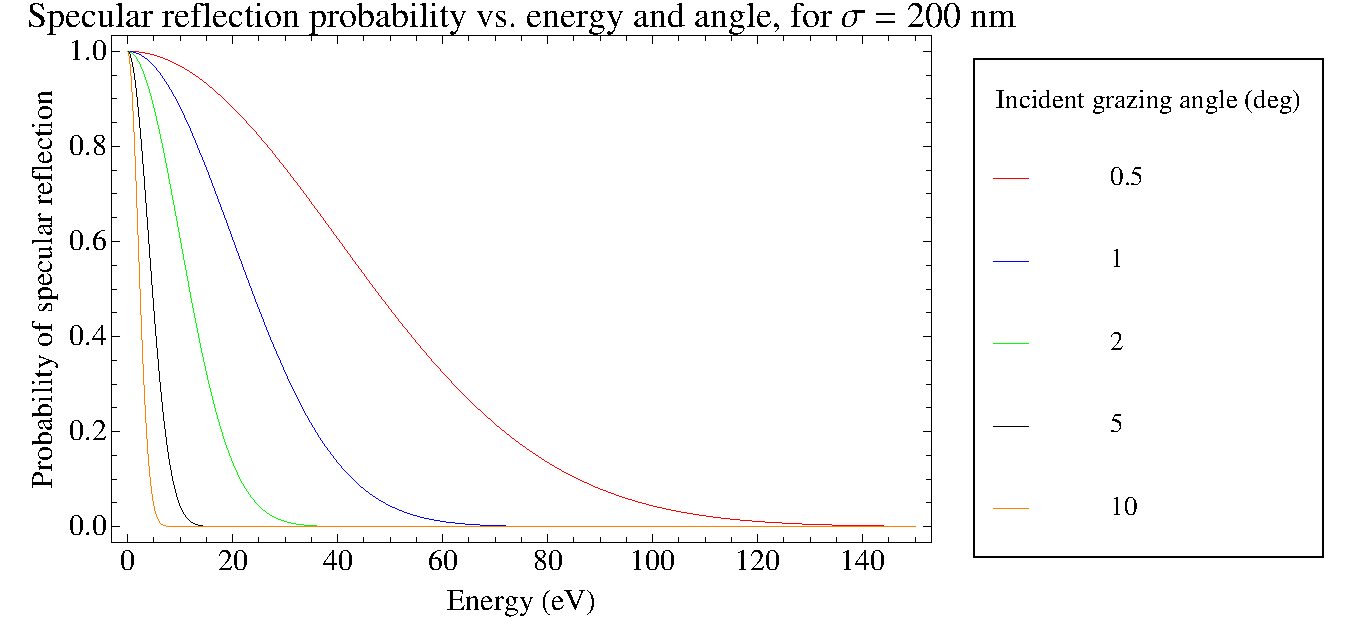
\includegraphics[width=6in]{Synrad3d/specular-probability.pdf}
  \caption[Specular reflection probability vs. photon energy and angle]
{\label{f:spec.prob}
Specular reflection probability~\cite{b:beckmann}, vs. photon energy
and angle, for an rms surface roughness of 200 nm.}
%\footnotesize{Picture taken from \citep{syn}}
  \end{figure}
   

The probability that a photon will reflect specularly from a surface depends on the the rms surface roughness $\sigma$, the wavelength of the photon $\lambda$, and the grazing angle. As shown in equation \ref{eq:SpRe}:
the formula for this probability is~\cite{b:beckmann}
   \begin{equation}
   \label{eq:SpRe}
P_{\textrm{spec}}=\textrm{e}^{-g(x,y)},
\end{equation}
where
   \begin{equation}
g(x,y)=\frac{4\pi^{2}\sigma^{2}(x+y)^{2}}{\lambda^{2}}
  \end{equation}
where $x$ is the cosine of the incident polar angle, and $y$ is the
cosine of the scattered polar angle.

For a typical technical vacuum chamber surface, the rms surface roughness $\sigma \gtrsim 200$ nm is
greater than most of the X-ray wavelengths of interest. In this regime diffuse scattering from the surface dominates over specular reflection. This is illustrated in Fig.~\ref{f:spec.prob}.
The model for diffuse scattering used by \srthree assumes a Gaussian distribution for both the surface height variations (rms $\sigma$) and for the transverse distribution.

The most general expression for the diffusely scattered power is complex, and involves an infinite sum.  However, the expression simplifies substantially in the limit $g(x,y)\gg 1.$ For very rough surfaces corresponding to technical vacuum chambers, for which typically $\sigma \gg \lambda$, this condition is satisfied over much of the region of interest.

\subsection{Input Files}
The input files used by \srthree are the following:
\subsubsection*{Synrad3D Main Input File (SMIF)}
\label{smif}
This file should be specified on the command line that invokes synrad3d, if it is not specified, it will select the default name "synrad3d.init". This file contains the parameters of the simulation
\begin{itemize}
\item The region where radiation is produced specified by the index numbers of elements in the lattice.
\item The direction in which the photons are travelling when initially created. 
\item The minimun number of photons that need to be generated before \srthree will stop the simulation.  
\item the number of photons generated throughout the radiation production region.
\item The minimun distance to track the particle beam between emission points.
\item The particle beam size.
\item The lattice file defining the optics of the accelerator.
\item The wall file defining the vacuum chamber's geometry.
\item The name of the output file.
\item The surface roughness for the default surface.
\item The surface roughness correlation for the default surface.
\item The surface reflection file for non-default surface.
\item The minimun and maximun initial energy values to be filtered by \srthree .
\end{itemize}
There are other parameters that can be specified in the SMIF, but are not mentioned here, because they are not relevant to this work.

\subsubsection*{Lattice File}
This file cointains the complete description of the elements of the lattice, defining the optics of the machine. This file must be specified in the SMIF.
\subsubsection*{Vacuum Chamber Wall Definition file}
The file specified in the SMIF defines the cross section of the vacuum chamber's wall at a number of longitudinal positions.
\subsubsection*{Chamber Surface Reflectivity file}
The reflectivity of the vacuum chamber wall can be described on the surface reflection file specified in the SMIF. If no file is specified \srthree will use the default reflectivity, which  is based on the refletivity of a Carbon film on Aluminum substrate. 

\subsection{Output Files}

\subsubsection*{Synrad3d Main Output File}
The name of this file must be specified in the SMIF. This file contains the information from the SMIF and the data generated for each photon. This information consists of:
\begin{itemize}
\item The number of the photon.
\item The number of times the photon hit the wall.
\item The photon energy.
\item The position where the photon was generated.
\item The position where the photon was absorbed.
\item The distance traveled by the photon.
\item The type of the lattice element where the photon was absorbed.
\end{itemize}

%----------------------------------------------------------------------------------------
%	SECTION 1
%----------------------------------------------------------------------------------------



%--------------------------------------------------------------------------------------------
\section{Tools}
Given the nature of routines described in \ref{Synrad3d}, using enough photons to obtain statistically valid results, running this program would take months in a regular commercial computer. To surpass this limitation the CERN {\it Lxplus} computing cluster was employed.
\subsection{Lxplus}
\label{lxplus}
The Lx Public Login Service or Lxplus is a login service offered to all CERN users. This cluster consists in several public machines running SLC5 in 64 bit mode, where all interactive and batch systems are built on top of the CERN standart Unix Enviroment. There is a wide range of shells available, that can be sorted in two groups: the C-shell like and the Bourne-shell like. We used Bash because of the full Linux based facilities. Since this machines are not to be used to store data a Workspace was made in the AFS file system that is accesible through normal system commands. Running CPU intense jobs in those machines is prohibited, so a system of jobs submissions to a set of queues with different limits on the available resources is at the disposal of the Lxplus user.
 
% Chapter Template

\chapter{Results} % Main chapter title

\label{Methodology} % Change X to a consecutive number; for referencing this chapter elsewhere, use \ref{ChapterX}

\lhead{Chapter 5. \emph{Results}} % Change X to a consecutive number; this is for the header on each page - perhaps a shortened title

%----------------------------------------------------------------------------------------
%	SECTION 1
%----------------------------------------------------------------------------------------

\section{Simulation}
We ran \srthree which was described in chapter \ref{soft}. Our aim was to simulate $10^{4}$ photons produced by a proton beam at 7 TeV energy. This amount of photons was used to balance a large enough number to present accurate statistical results and the amount of available computing time, but because of technical challenges mentioned in subsection \ref{lxplus}, we divided the simulation into several simulations with a much smaller number of photons, there were simulations with 10, 20 and 50 photons each, which we can join together because photons do not interact with each other.



%-----------------------------------
%	SUBSECTION 1
%-----------------------------------
\subsection{SMIF}
The SMIF used to run this simulations used the following parameters:
\begin{itemize}
\item The wall file describing the vacuum chamber with a sawtooth pattern, of a series of 30 $\mu$m high steps at adistance of 500 $\mu$m in the longitudinal direction, which is on the horizontal. (sawtoohTEST.wall). The transversal section of the beam screen is shown in Figure \ref{fig:xy}.

\begin{figure}
	\centering
  \begin{minipage}{\textwidth}
  	\centering
   	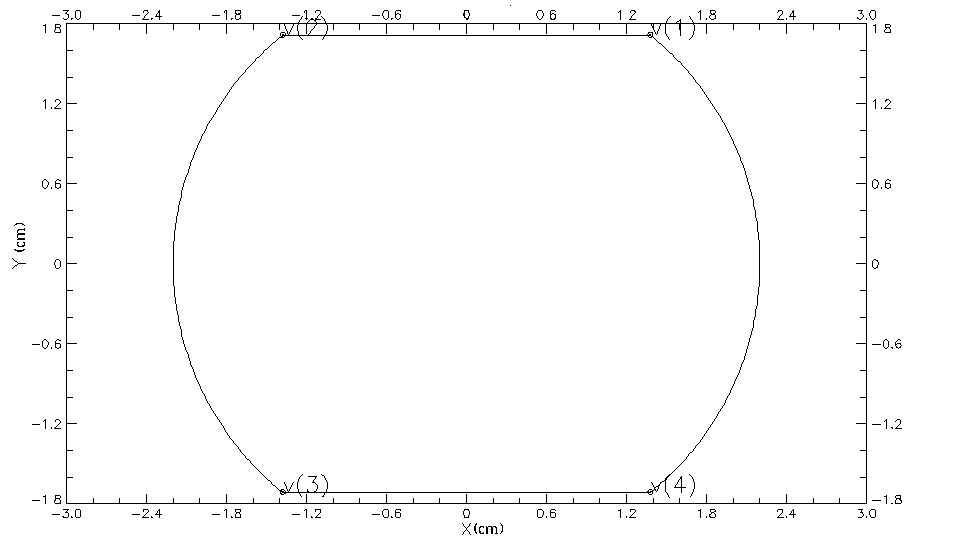
\includegraphics[width=5.5in]{Pictures/transsect.jpg}
  		\caption{\label{fig:xy}
   			Transversal section of the beam screen in the cold arcs. }
   			\footnotesize{Image plotted with \srthree}
   \end{minipage}
\end{figure}
\item The lattice file which contains the version 6.5 of the LHC was employed. (V6.5.out.bmad)
\item The starting element was set to be 142 and the ending element 146. All elements inside that range are bending dipoles.
\item The photon direction was set to be positive wich means a forward generation.
\item The number of photons varied between 10, 20 and 50.
\item The seed for the random number generator was set to be the system clock.
\item A custom reflectivity table was used. (reflectivity.table.C.CU.dat). This table assumes a carbon layer of 10 nm on a copper substrate. For this table the probability of reflection ($P_{\textrm{reflect}}$) was taken from the LBNL X-ray database\cite{lbnl}.
\end{itemize} 

%-----------------------------------
%	SUBSECTION 2
%-----------------------------------

\subsection{SMOF}
After all simulations were run through the batch system the results were concatenated into a single file containing a single table with the information of 9,227 photons that where generated, and absorbed by the beam screen between sections 142 and 146.


%----------------------------------------------------------------------------------------
%	SECTION 2
%----------------------------------------------------------------------------------------
\subsection{Secondary Simulation}
In order to have data to compare to the data we obtained, we ran a single simulation featuring $10^4$ photons using the same parameters except the sawtooth pattern of the wall file. In other words we simulated with the same parameters but with a smooth beam pipe. We kept the first 9,227 photons just to have the same number of photons in both simulations.

\subsection{Analysis}
In both simulations all photons were absorbed in the last element analyzed (bending magnet 146) with no rebounds. The exact position where photons were absorbed are shown in Figure \ref{fig:s}. Figure \ref{fig:s} shows an histogram of photons absorbed versus the position on the s axis, The ones from the sawtooth pattern simulation is are shown in red, and the ones from the smooth surface simulation in blue.
\begin{figure}%[ht]
%\centering % used for centering table
 % \begin{minipage}{\textwidth}
  	\centering
   	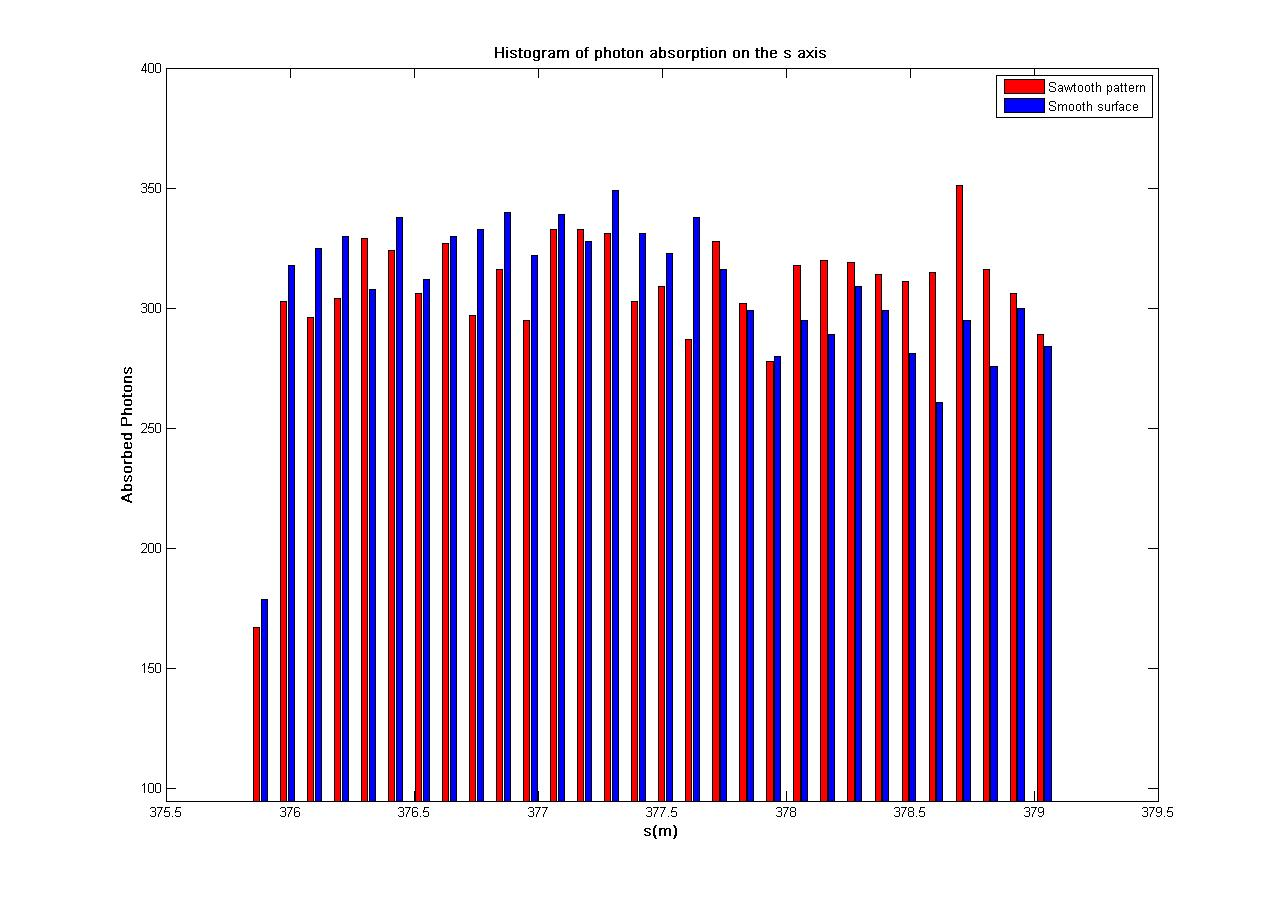
\includegraphics[width=6.5in, height=.65\textheight]{Graficas/nuevas/sbarras.jpg}
  		\caption{\label{fig:s}
   			Position on the s axis where photons were absorbed.}
%   			\footnotesize{Image plotted with \srthree}
  % \end{minipage}
 \end{figure}


The energies at which photons were absorbed are shown in Figure \ref{fig:energia}. It shows in blue the results for the primary simulation and in red the result for the secondary simulation. The mean energy from all photons absorbed by the sawtooth pattern is 27.109 eV and 27.113 for the smooth surface.  

\begin{figure}%[ht]
%\centering % used for centering table
%  \begin{minipage}{\textwidth}
  	\centering
   	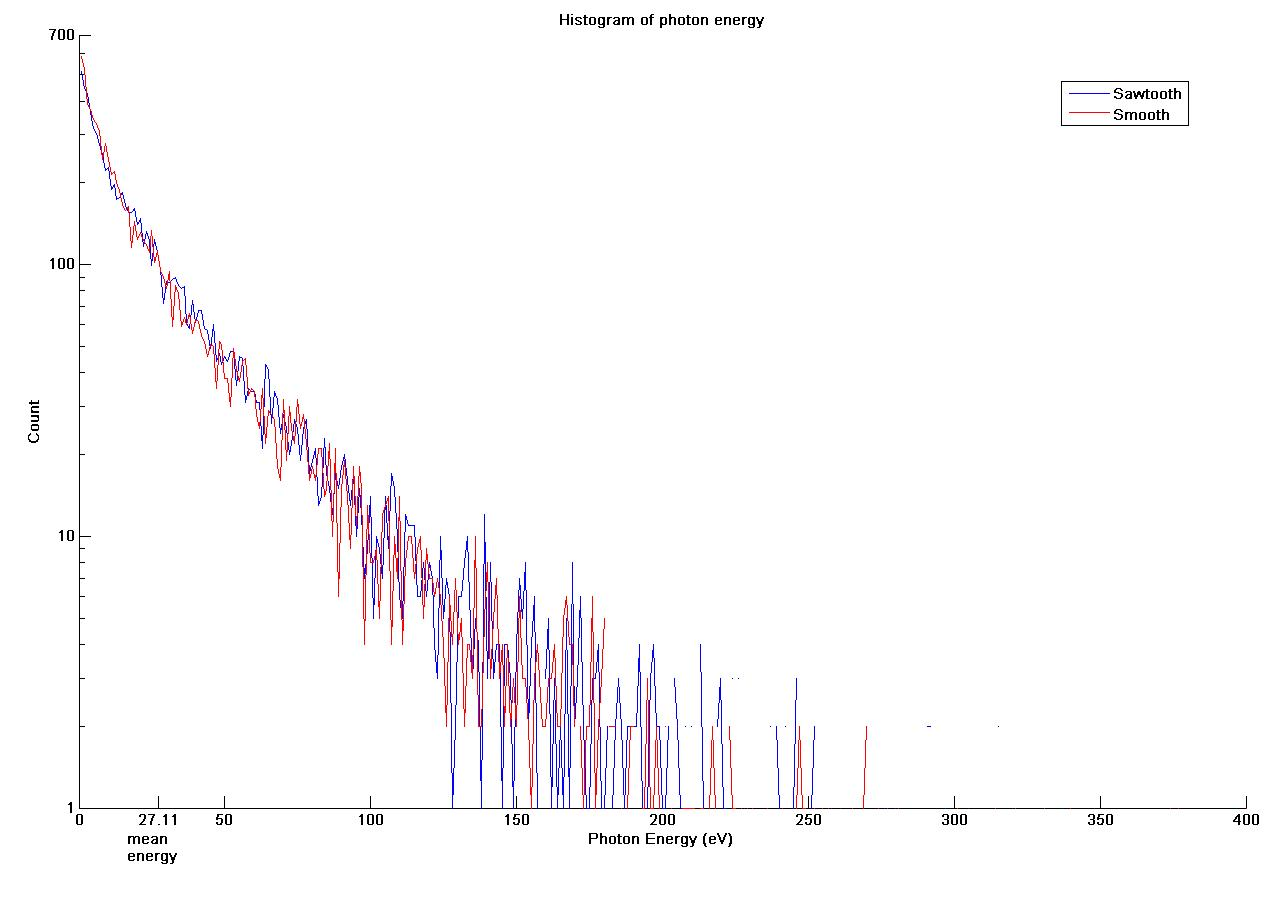
\includegraphics[width=6.5in, height=.65\textheight]{Graficas/nuevas/energias.jpg}
  		\caption{\label{fig:energia}
   			Energy of absorbed photons. }
%   			\footnotesize{Image plotted with \srthree}
 %  \end{minipage}
\end{figure}



An histogram for the position X-Y where photons were absorbed are shown in Figure \ref{fig:xy} for the main simulation and Figure \ref{fig:xyplana} for the smooth beam pipe. 
\begin{figure}

%\centering % used for centering table
%  \begin{minipage}{\textwidth}
  	\centering
   	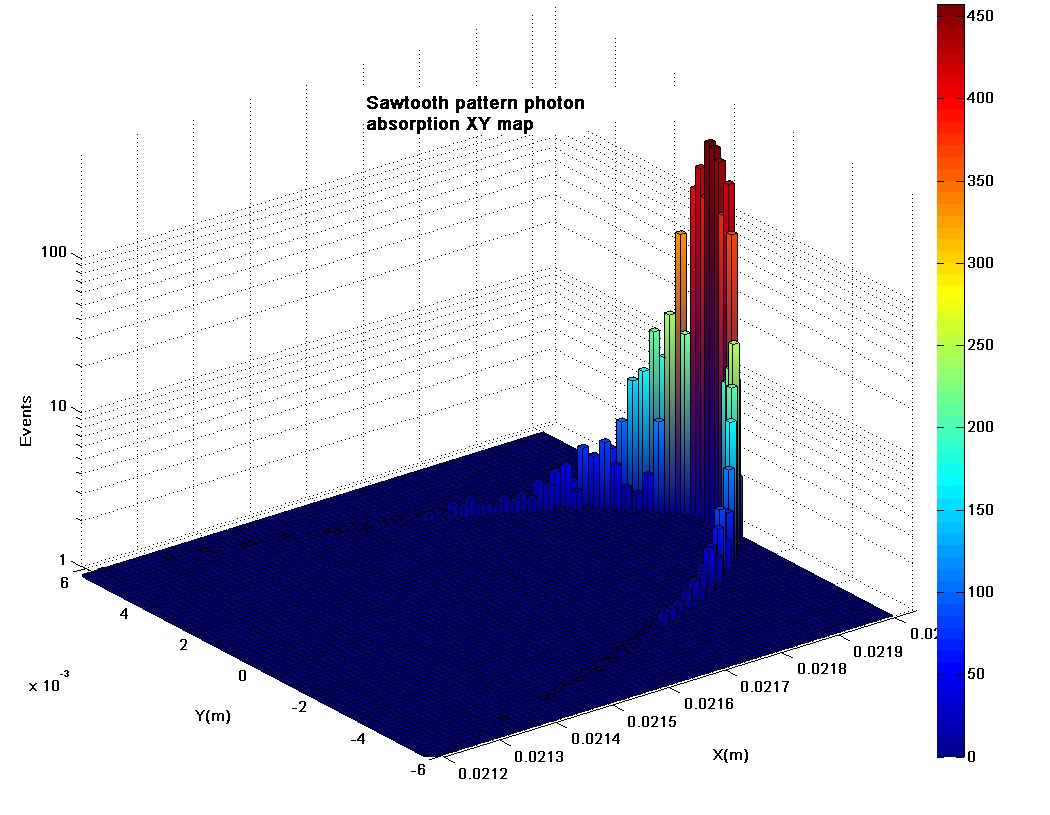
\includegraphics[height=.45\textheight]{Graficas/nuevas/xy.jpg}
  		\caption{\label{fig:xy}
   			 X-Y absorption points for the sawtooth pattern beam screen.}
%   			\footnotesize{Image plotted with \srthree}
 %  \end{minipage}
\end{figure}   

 \begin{figure}
 
  % \begin{minipage}{\textwidth}
  	\centering
   	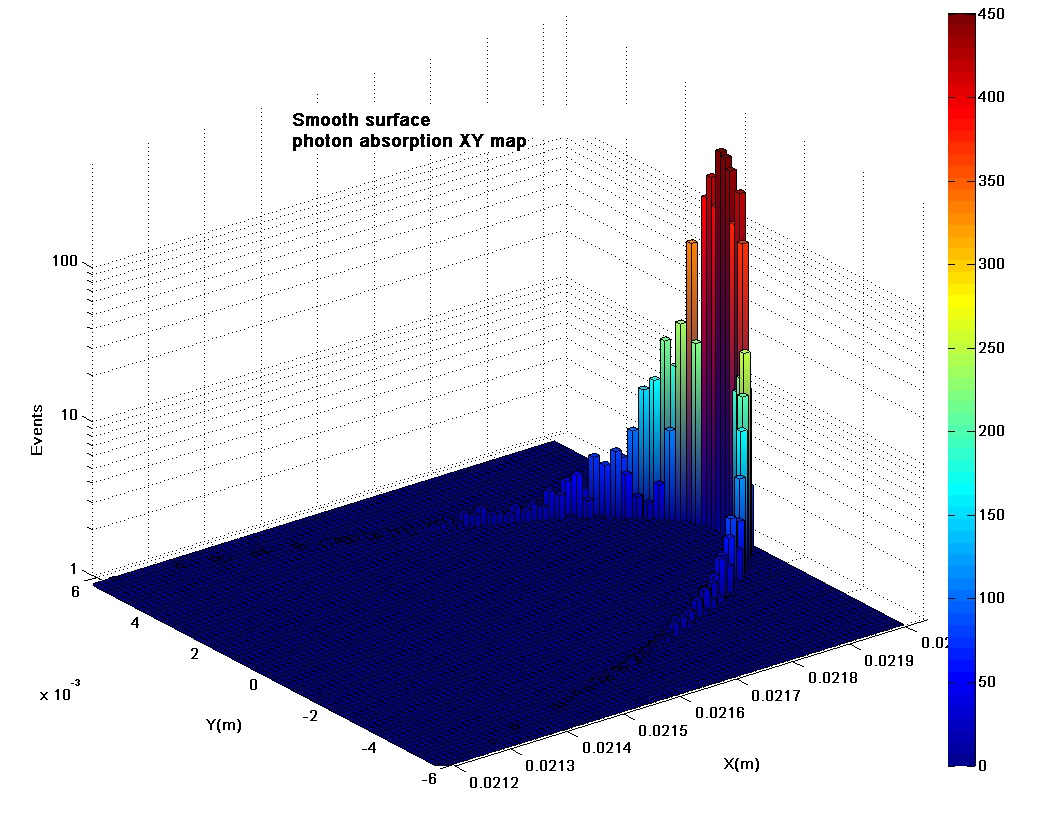
\includegraphics[height=.45\textheight]{Graficas/nuevas/smoothxy.jpg}
  		\caption{\label{fig:xyplana}
   			X-Y absorption points for the smooth surface beam screen.}
%   			\footnotesize{Image plotted with \srthree}
%\end{minipage}
%\label{comp:3} % is used to refer this table in the text
\end{figure}



 
%% Chapter Template

\chapter{Chapter Title Here} % Main chapter title

\label{ChapterX} % Change X to a consecutive number; for referencing this chapter elsewhere, use \ref{ChapterX}

\lhead{Chapter X. \emph{Chapter Title Here}} % Change X to a consecutive number; this is for the header on each page - perhaps a shortened title

%----------------------------------------------------------------------------------------
%	SECTION 1
%----------------------------------------------------------------------------------------

\section{Main Section 1}

Lorem ipsum dolor sit amet, consectetur adipiscing elit. Aliquam ultricies lacinia euismod. Nam tempus risus in dolor rhoncus in interdum enim tincidunt. Donec vel nunc neque. In condimentum ullamcorper quam non consequat. Fusce sagittis tempor feugiat. Fusce magna erat, molestie eu convallis ut, tempus sed arcu. Quisque molestie, ante a tincidunt ullamcorper, sapien enim dignissim lacus, in semper nibh erat lobortis purus. Integer dapibus ligula ac risus convallis pellentesque.

%-----------------------------------
%	SUBSECTION 1
%-----------------------------------
\subsection{Subsection 1}

Nunc posuere quam at lectus tristique eu ultrices augue venenatis. Vestibulum ante ipsum primis in faucibus orci luctus et ultrices posuere cubilia Curae; Aliquam erat volutpat. Vivamus sodales tortor eget quam adipiscing in vulputate ante ullamcorper. Sed eros ante, lacinia et sollicitudin et, aliquam sit amet augue. In hac habitasse platea dictumst.

%-----------------------------------
%	SUBSECTION 2
%-----------------------------------

\subsection{Subsection 2}
Morbi rutrum odio eget arcu adipiscing sodales. Aenean et purus a est pulvinar pellentesque. Cras in elit neque, quis varius elit. Phasellus fringilla, nibh eu tempus venenatis, dolor elit posuere quam, quis adipiscing urna leo nec orci. Sed nec nulla auctor odio aliquet consequat. Ut nec nulla in ante ullamcorper aliquam at sed dolor. Phasellus fermentum magna in augue gravida cursus. Cras sed pretium lorem. Pellentesque eget ornare odio. Proin accumsan, massa viverra cursus pharetra, ipsum nisi lobortis velit, a malesuada dolor lorem eu neque.

%----------------------------------------------------------------------------------------
%	SECTION 2
%----------------------------------------------------------------------------------------

\section{Main Section 2}

Sed ullamcorper quam eu nisl interdum at interdum enim egestas. Aliquam placerat justo sed lectus lobortis ut porta nisl porttitor. Vestibulum mi dolor, lacinia molestie gravida at, tempus vitae ligula. Donec eget quam sapien, in viverra eros. Donec pellentesque justo a massa fringilla non vestibulum metus vestibulum. Vestibulum in orci quis felis tempor lacinia. Vivamus ornare ultrices facilisis. Ut hendrerit volutpat vulputate. Morbi condimentum venenatis augue, id porta ipsum vulputate in. Curabitur luctus tempus justo. Vestibulum risus lectus, adipiscing nec condimentum quis, condimentum nec nisl. Aliquam dictum sagittis velit sed iaculis. Morbi tristique augue sit amet nulla pulvinar id facilisis ligula mollis. Nam elit libero, tincidunt ut aliquam at, molestie in quam. Aenean rhoncus vehicula hendrerit. 
% Chapter Template

\chapter*{Conclusion} % Main chapter title
\addcontentsline{toc}{chapter}{Conclusion}
\label{conclusion} % Change X to a consecutive number; for referencing this chapter elsewhere, use \ref{ChapterX}

\lhead{\emph{Conclusion}} % Change X to a consecutive number; this is for the header on each page - perhaps a shortened title
%----------------------------------------------------------------------------------------
%	SECTION 1
%----------------------------------------------------------------------------------------

No big difference between the Sawtooth Pattern beam screen and the smooth one were observed in both the position in the transversal direction (s) and energy of the absorbed photons (Figures \ref{fig:s}$-$\ref{fig:energia}). The difference that do appear, are only statistical error. I strongly believe this is because none of the photons bounced off the screen.

The simulation considering a sawtooth pattern in the beam screen showed a more extended distribution on the X-Y map Figure \ref{fig:xy} than the one on smooth screen \ref{fig:xyplana}. This can make the cooling process more efficient.

Considering all this, the main conclusion is that the length we need to consider in our simulations should be longer than threee elements to really appreciate the difference the sawtooth pattern on the beam screen makes. But this simulation does help us to notice that in small accelerators having a sawtooth pattern on te beam screen would help us a little to nothing.
\section*{Future Work} % Main chapter title
\addcontentsline{toc}{section}{Future Work}
\label{FW}
The first step is to share our result with people at CERN, and compare with measurements. 
There are also two further steps that must be taken in the future to complete this work.
The first one is to take an arc section long enough for photons to bounce at least two times in order to make the differences more noticeable. 
The second one is to take the whole arc into account, this will help us pinpoint the sections that suffer more heating due to synchrotron radiation and will help us fully understand how the sawtooth pattern help us distributing the heat produced by SR and to reduce the primary emmision of electrons that would give rise to an electron cloud. And then back to sharing the resuts with CERN and comparing to measurements. 

%----------------------------------------------------------------------------------------
%	THESIS CONTENT - APPENDICES
%----------------------------------------------------------------------------------------

\addtocontents{toc}{\vspace{2em}} % Add a gap in the Contents, for aesthetics

\end{document}  
